\section{Лекция (Вероятностные Модели)}

\subsection{Вероятностные модели $(\Omega, \F, \Pb)$}

\subsubsection{Дискретные Модели}
\[ |\Omega| < \infty \qquad \F = 2^\Omega\]

Бывают двух типов:
\begin{enumerate}
    \item Классические модели
        \[ p(\omega i) = const \qquad \Pb (A) = \frac{|A|}{|\Omega|} \]
    \item Неклассическая модель
\end{enumerate}

\textbf{Урновая схема}: $n$ шариков и вытаскиваете $k$. Есть несколько типов:
\begin{enumerate}
\item Упорядоченная выборка с возвращением
    \[\Omega = \{(i_1, \ldots, i_k), \; 1 \leq i_j \leq n\} \qquad |\Omega| = n^k\text{, классическая}\]

\item Упорядоченная выборка без возвращения
    \[\Omega = \{(i_1, \ldots, i_k), \; i_j \neq i_m, j \neq m, 1 \leq i_j \leq n\} \qquad |\Omega| = A^k_n\text{, классическая}\]

\item Неупорядоченная выборка без возвращения
    \[ \Omega = \{ \{i_1, \ldots, i_k\} \;|\; i_j \neq i_m, j\neq m, \; 1\leq j \leq n\} \qquad |\Omega| = \frac{A_n^k}{k!}=C_n^k\text{, классическая} \]

\item Неупорядоченная выборка с возвращением

    То есть у нас есть $k$ элементов, которые могут еще и повторяться.
    \[ \Omega = \left\{ (m_1, \ldots, m_n) \;|\; \sum_{i=1}^nm_i=k\right\} = \{(\epsilon_1,\ldots, \epsilon_{n+k-1}) \;|\; \epsilon_i \in \{0,1\}, n-1\text{ единиц}\} \]
где $m_i$~--- число шариков с номером  $i$ в нашей выборке. Равенство выводится методом перегородок, где перегородками являются $n-1$ единиц.
\[ |\Omega| =  C^{n-1}_{n+k-1}, \quad \text{история неклассическая} \]
Неклассическая потому что, например, если доставать два шарика из двух шариков (красный и белый), то случай с двумя красными будет выпадать в два раза реже, чем красный и белый.
\begin{gather*}
P((m_1, \ldots, m_n))  = \frac{\text{\#упор. набор}: (m_1,\ldots,m_n)}{n^k} =\\
\frac{C_k^{m_1}\cdot C_{k-m_1}^{m_2} \cdot C_{k-m_1-m_2}^{m3}\cdot \ldots}{n^k} = 
\frac{k!}{m_1!m_2!\ldots m_n!\cdot n!} 
\end{gather*}

\end{enumerate}

\begin{problem}
    Есть $M$-white и $(N-M)$ black шаров. Упорядоченная выборка с возвращением размера $n$. Найти вероятность конкретной последовательности цветов $(\alpha_1,\ldots, \alpha_n)$.   
\end{problem}
\begin{proof}
White $= \{0\}$, Black $= \{1\}$
    
$N$ чисел 
\begin{gather*}
\omega = (i_1,\ldots, i_n) \qquad 1 \leq i_j \leq N\\
i_1 \ldots i_M \text{ --- white} \qquad
i_{M+1} \ldots i_N \text{ --- black} \\
|\Omega| = N^n\\
N_b = \sum_{i=1}^n \alpha_i \qquad N_w = n-N_b \\
|A| = M^{N_w} \cdot (N-M)^{N_b} \\
\Pb(A) = \frac{M^{N_w} \cdot (N-M)^{N_b}}{N^n} = 
\left( \frac{M}{N} \right)^{n - \sum \alpha_i} \cdot \left( \frac{N-M}{N}\right)^{\sum\alpha_i} = \\
\left\{\frac{N-M}{N}=p\in(0;1)\right\} =
p^{\sum\alpha_i}(1-p)^{n-\sum\alpha_i}
\end{gather*}

Вторая Модель (схема испытаний Бернулли) 

 \begin{gather*}
     \omega = (\alpha_i,\ldots,\alpha_n) \quad
     p(w) = p^{\sum\alpha_i}(1-p)^{n-\sum\alpha_i}
 \end{gather*}
\end{proof}

\subsection{Схема испытаний Бернулли}
Есть последовательность $\omega = (\alpha_i,\ldots,\alpha_n)$ одинаковых экспериментов и всего два результата $\alpha_i \in \{0;1\}$, $p$~--- вероятность единицы.
\[ p(\omega) = p^{\sum\alpha_i}\cdot(1-p)^{n-\sum\alpha_i} \]

Чтобы убедится, что это правда вероятностная модель нужно проверить получится ли единица в результате суммирования всех вероятностей по всем исходам.

\begin{gather*}
    \sum_{\omega\in\Omega}p(\omega)=
    \sum_{k=0}^n \quad \cdot \sum_{\omega:\sum_{i=1}^n\alpha_i=k} p(\omega) =
    \sum_{k=0}^np^k (1 - p)^{n-k} C_n^k = (p + (1 - p))^n = 1
\end{gather*}


Теперь представим другой эксперимент. Решка~--- 1, орел~--- 0. Хочется построить модель.
\begin{example}
Кидаем монетку до орла. В нашем случае $\omega = k$, где $k$~--- номер броска, на котором выпал номер броска впервые.
\begin{gather*}
    p(\omega) = p^{k-1}(1-p)\\
    \sum p(\omega) = \sum_{k=1}^\infty p^{k-1}(1-p) = 1 - p\frac{1}{1-p} = 1
\end{gather*}

\end{example}

Проблема: Непонятно что делать, если $|\Omega| = \infty$, поскольку тогда сумма не может быть посчитана (т.к. пропадает счётность).

\subsection{Недискретные модели}

\begin{problem}\label{pr:2.2}
О встрече. Два друга договорились о встрече в промежутке от 12 до 13 часов. Каждый ждет не более 15 минут.
Найти вероятность встречи.
\end{problem}

\begin{proof}
\begin{gather*}
    \omega = (i_1,i_2) \qquad  i\text{~--- время прихода}  \\
    A = |i_1 - i_2| < \frac{1}{4} \\
    \Pb(A)= \frac{1-8\cdot0,5\cdot0,75 \cdot 0,75}{1} = \frac{7}{16}\\
    \Omega = \{(i_1, i_2), \; 0 \leq i_j \leq 1 \} \qquad \F = 2^\Omega\\
    \Pb(A) = \frac{\mu(A)}{\mu(\Omega)}
\end{gather*}

\begin{figure}[ht]
    \centering
    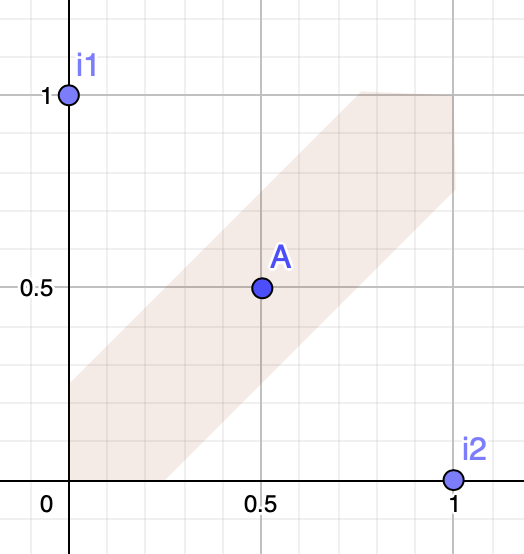
\includegraphics[width=0.4\textwidth]{img1}
    \caption{К задаче \ref{pr:2.2}}
    \label{fig:1}
\end{figure} 
Была упомянута проблема определения $p(A)$, поскольку, даже если взять за $\mu$ меру Лебега, все равно останутся неизмеримые подмножества.
\end{proof}

\subsection{Условная Вероятность $(\Omega, \F, \Pb)$}
%Рассмотрим на примере покера. $\omega = (i_1, \ldots, i_5, i_6, i_7)$

\begin{gather*}
    \Pb(A|B) = \frac{|A\cap B|}{|B|} = \frac{\Pb(A\cap B)}{\Pb(B)} \text{ классическая модель}
\end{gather*}

\begin{definition}
    \textbf{Условная вероятность} (в дискретном случае) $A$ относительно $B$, если $P(B)\neq 0$, определяется:
\begin{equation}
\Pb(A|B) =  \frac{\Pb(A\cap B)}{\Pb(B)}.
\end{equation}
\end{definition}

\begin{example}
Схема Бернулли.

Хотим найти вероятность того, что в эксперименте, в котором выбираются $n$ случаев первый будет успешным, при условии того, что всего успешных случаев $k$.
\begin{gather*}
    B = k \text{ успехов} \qquad A = 1 \text{-й успех}\\ 
    \Pb(A\cap B) = \sum_{\substack{\omega:\; \alpha_1 = 1\\ \sum\alpha_i =k}} p(\omega) = 
    \{p(\omega) = p^k(1-p)^{n-k}\} =
    p^k(1-p)^{n-k} \cdot C_{n-1}^{k-1}\\
    \Pb(B) = C_n^k \cdot p^k(1-p)^{n-k}\\
    \Pb(A|B) = \frac{C_{n-1}^{k-1}}{C_n^k} = \frac{k}{n}
\end{gather*}
Получили ответ, который был интуитивно очевиден с самого начала.
\end{example}
